\chapter{Evolución lineal de los campos} \label{sec:cap3}

\section{Resonancia Paramétrica}

\begin{figure}[htbp]
    \centering
    \begin{subfigure}[t]{0.75\linewidth}
        \centering
        
\includegraphics[width = \linewidth]{figures/background_m2phi2.pdf}
        \subcaption{$m^2 \phi^2$}
    \end{subfigure}
    \begin{subfigure}[b]{0.75\linewidth}
        \centering
        
\includegraphics[width = \linewidth]{figures/Background_lphi4.pdf}
        \subcaption{$\lambda \phi^4$}
    \end{subfigure}
    \caption{}
    \label{fig:Floquet}
\end{figure}


\section{Análisis de Floquet}

\begin{figure}[htbp]
    \centering
    \begin{subfigure}[t]{0.75\linewidth}
        \centering
        
\includegraphics[width = \linewidth]{figures/Floquet_m2phi2.pdf}
        \subcaption{$m^2 \phi^2$}
    \end{subfigure}
    \begin{subfigure}[b]{0.75\linewidth}
        \centering
        
\includegraphics[width = \linewidth]{figures/Floquet_lphi4.pdf}
        \subcaption{$\lambda \phi^4$}
    \end{subfigure}
    \caption{}
    \label{fig:Floquet}
\end{figure}

\begin{figure}[htbp]
    \centering
    \begin{subfigure}[l]{0.45\linewidth}
        \centering
        
\includegraphics[width = \linewidth]{figures/narrow_resonance_m2phi2.pdf}
        \subcaption{Narrow resonance: amplitud}
    \end{subfigure}
    \begin{subfigure}[r]{0.45\linewidth}
        \centering
        
\includegraphics[width = \linewidth]{figures/broad_resonance_m2phi2.pdf}
        \subcaption{Broad resonance: amplitud}
    \end{subfigure}
    \begin{subfigure}[l]{0.45\linewidth}
        \centering
        \includegraphics[width = \linewidth]{figures/nk_Narrow_resonance_m2phi2.pdf}
        \subcaption{Narrow resonance: número de ocupación}
    \end{subfigure}
    \begin{subfigure}[r]{0.45\linewidth}
        \centering
        \includegraphics[width = \linewidth]{figures/nk_Broad_resonance_m2phi2.pdf}
        \subcaption{Broad resonance: número de ocupación}
    \end{subfigure}
    \caption{}
    \label{fig:m2phi2_Resonance}
\end{figure}

\begin{figure}[htbp]
    \centering
    \begin{subfigure}[l]{0.45\linewidth}
        \centering
        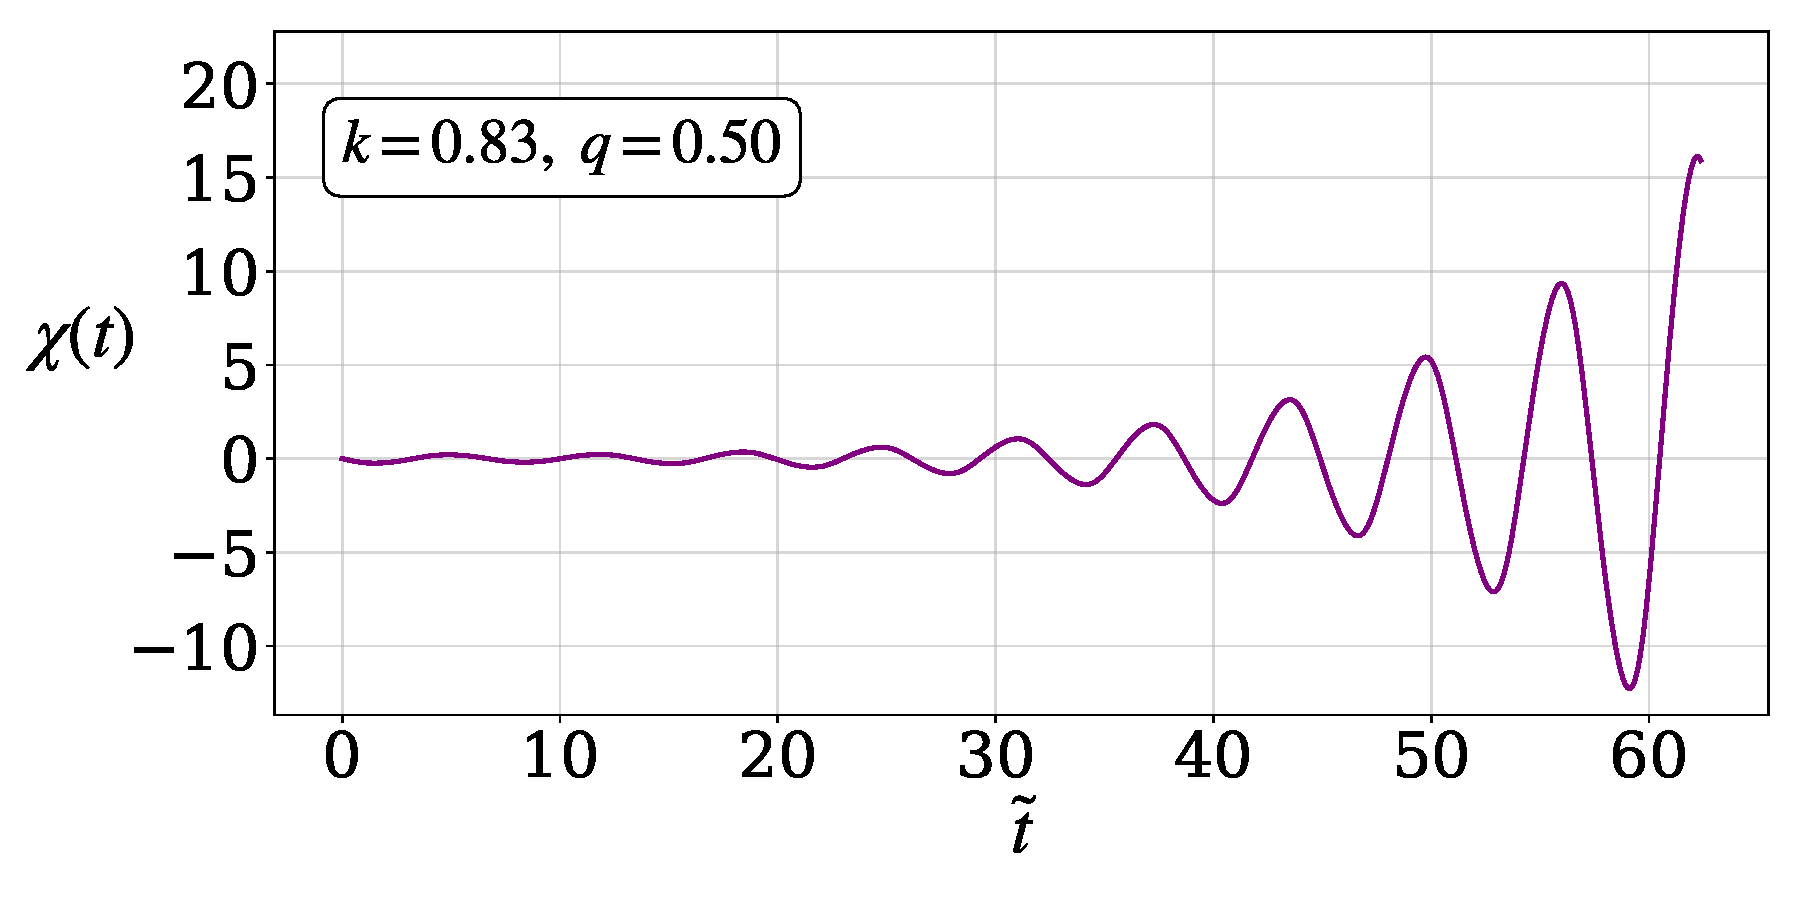
\includegraphics[width = \linewidth]{figures/Narrow_Resonance_lphi4.pdf}
        \subcaption{Narrow resonance: amplitud}
    \end{subfigure}
    \begin{subfigure}[r]{0.45\linewidth}
        \centering
        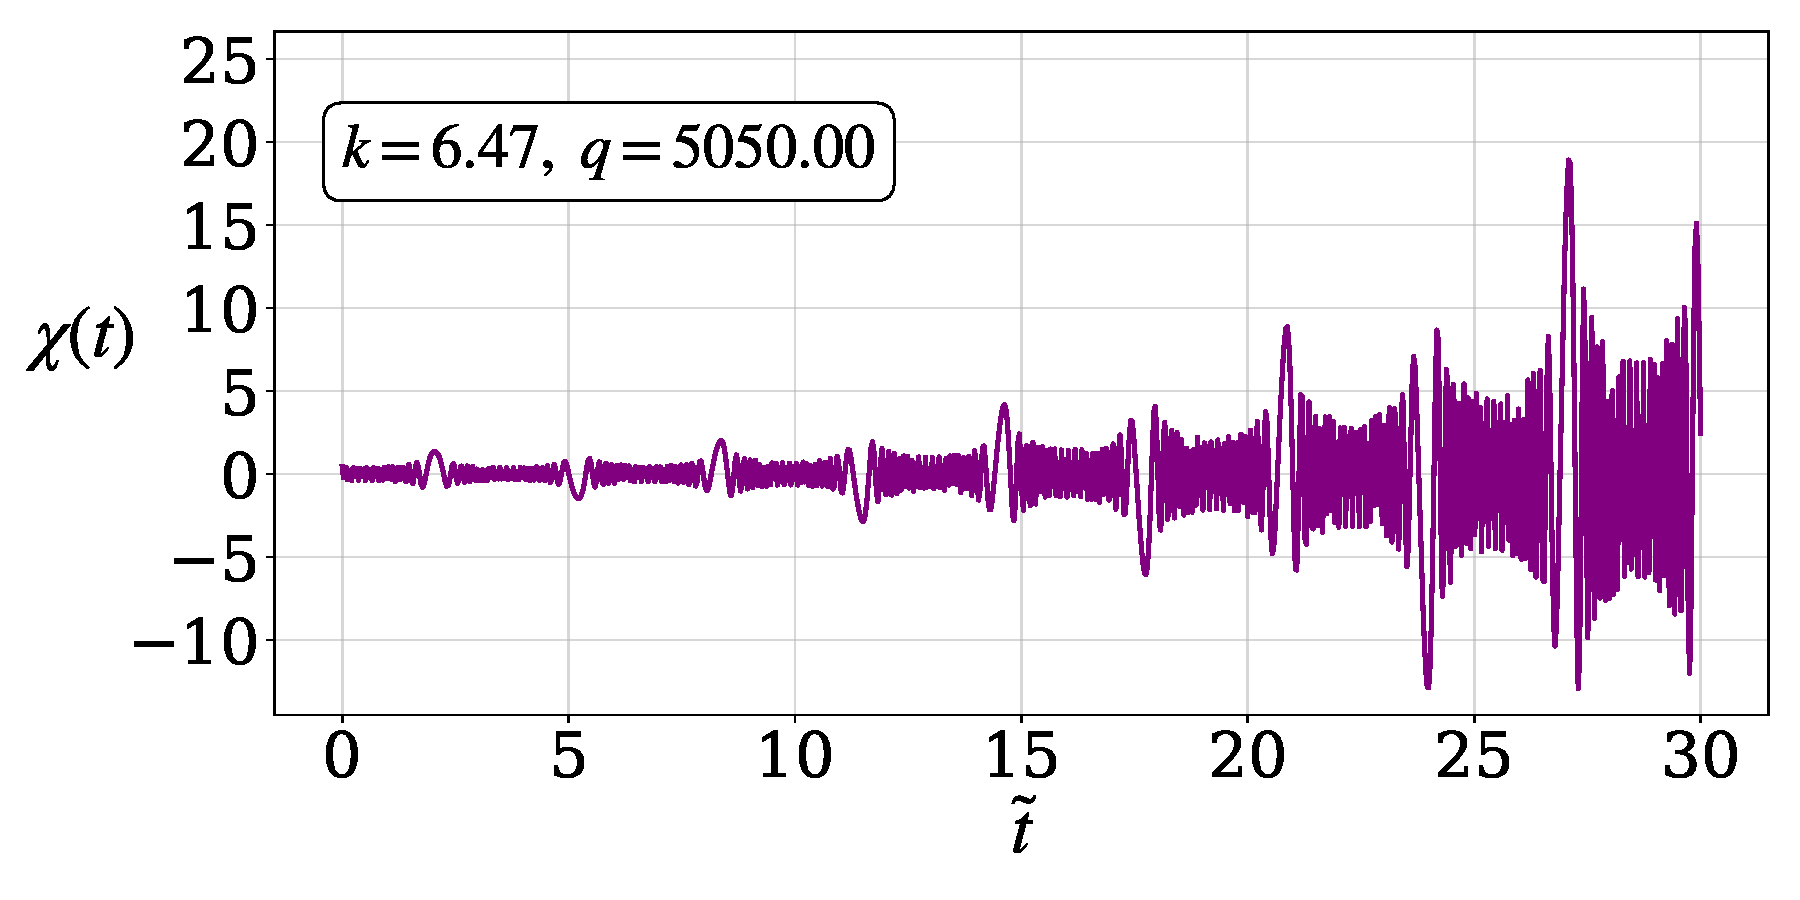
\includegraphics[width = \linewidth]{figures/Broad_Resonance_lphi4.pdf}
        \subcaption{Broad resonance: amplitud}
    \end{subfigure}
    \begin{subfigure}[l]{0.45\linewidth}
        \centering
        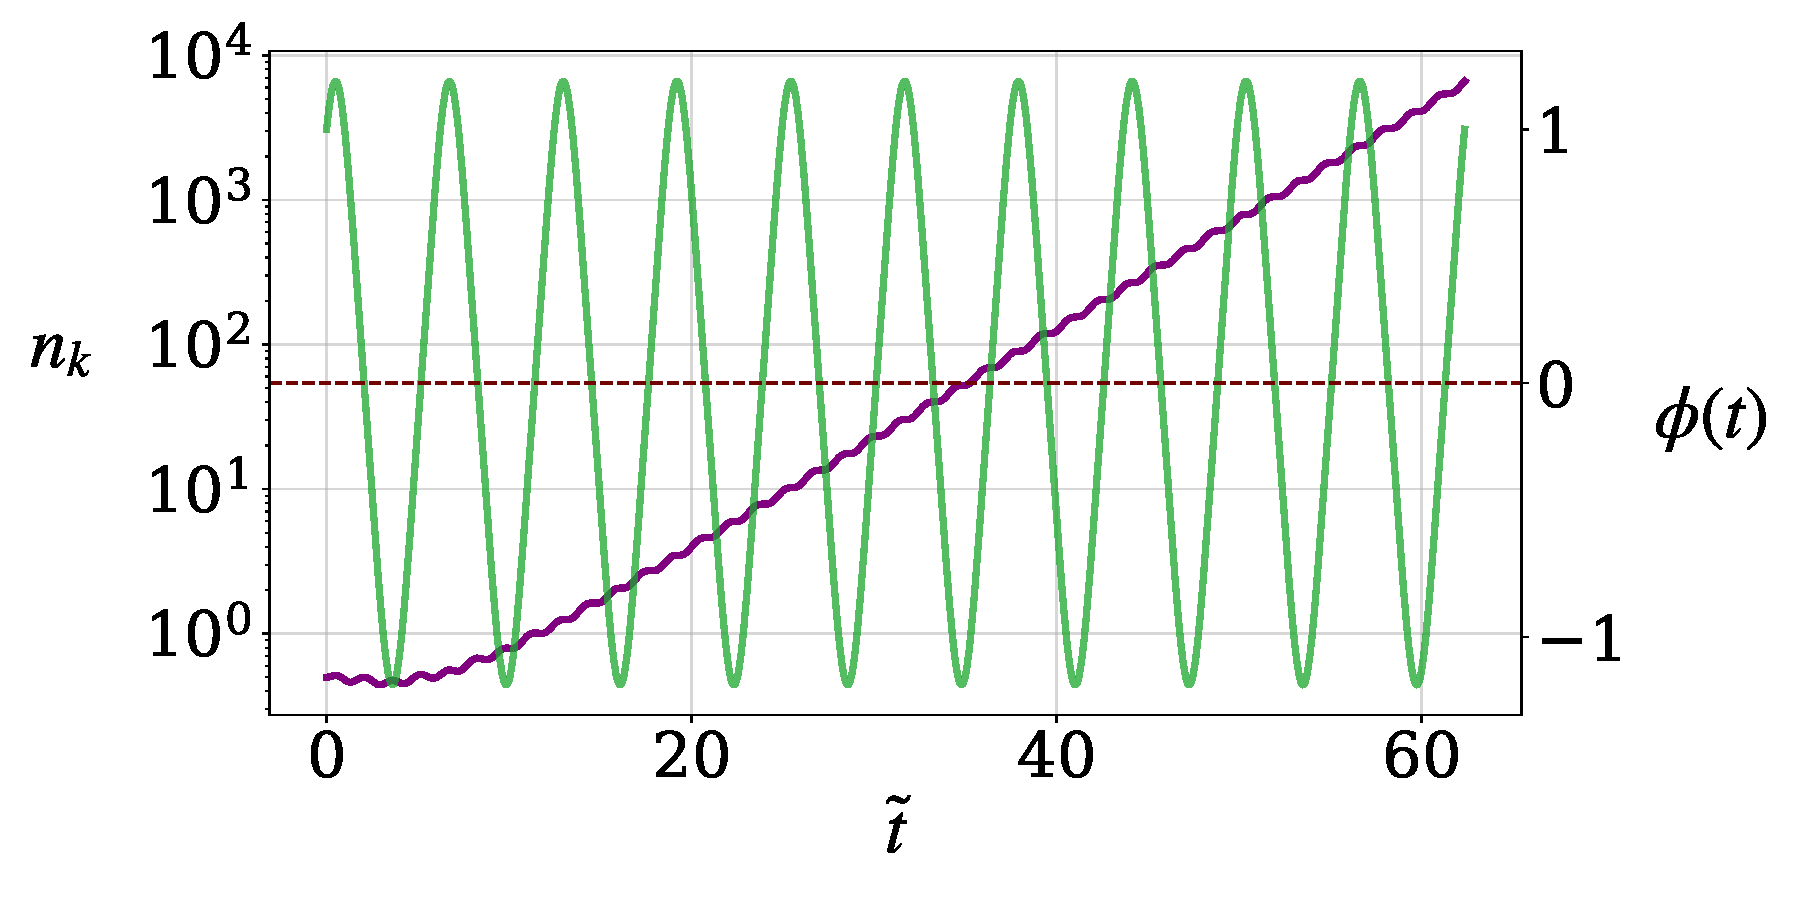
\includegraphics[width = \linewidth]{figures/nk_Narrow_Resonance_lphi4.pdf}
        \subcaption{Narrow resonance: número de ocupación}
    \end{subfigure}
    \begin{subfigure}[r]{0.45\linewidth}
        \centering
        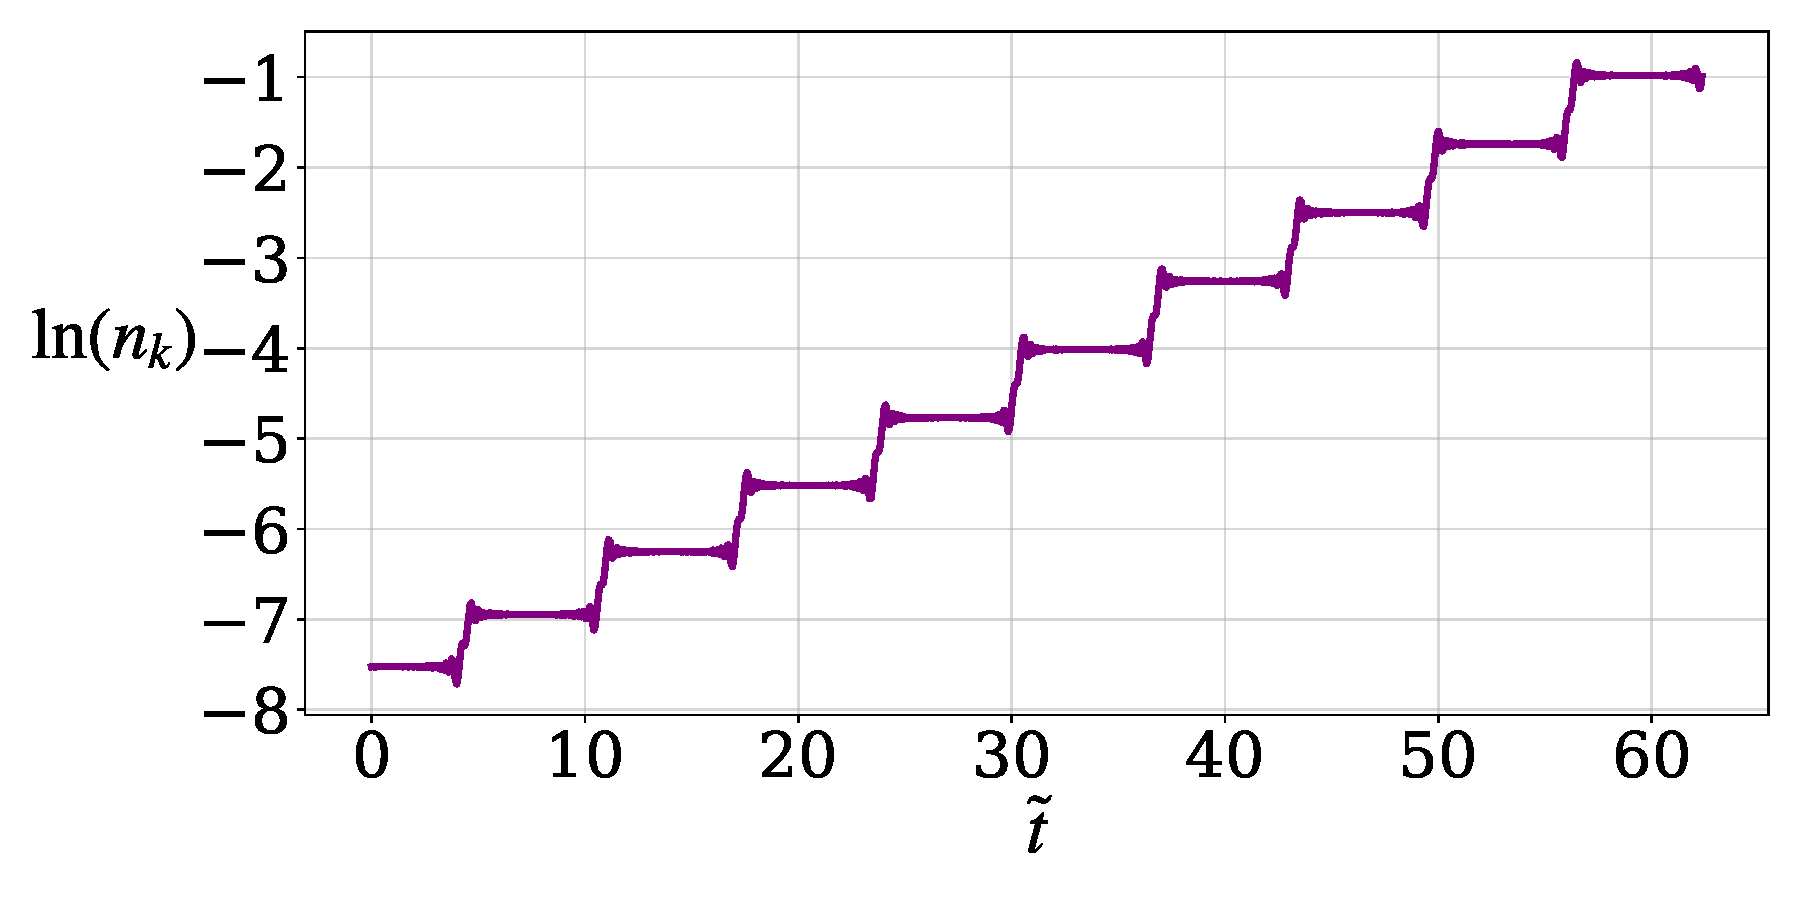
\includegraphics[width = \linewidth]{figures/nk_Broad_Resonance_lphi4.pdf}
        \subcaption{Broad resonance: número de ocupación}
    \end{subfigure}
    \caption{}
    \label{fig:lphi4_Resonance}
\end{figure}

\section{Producción lineal de ondas gravitacionales}

\begin{figure}[htbp]
    \centering
    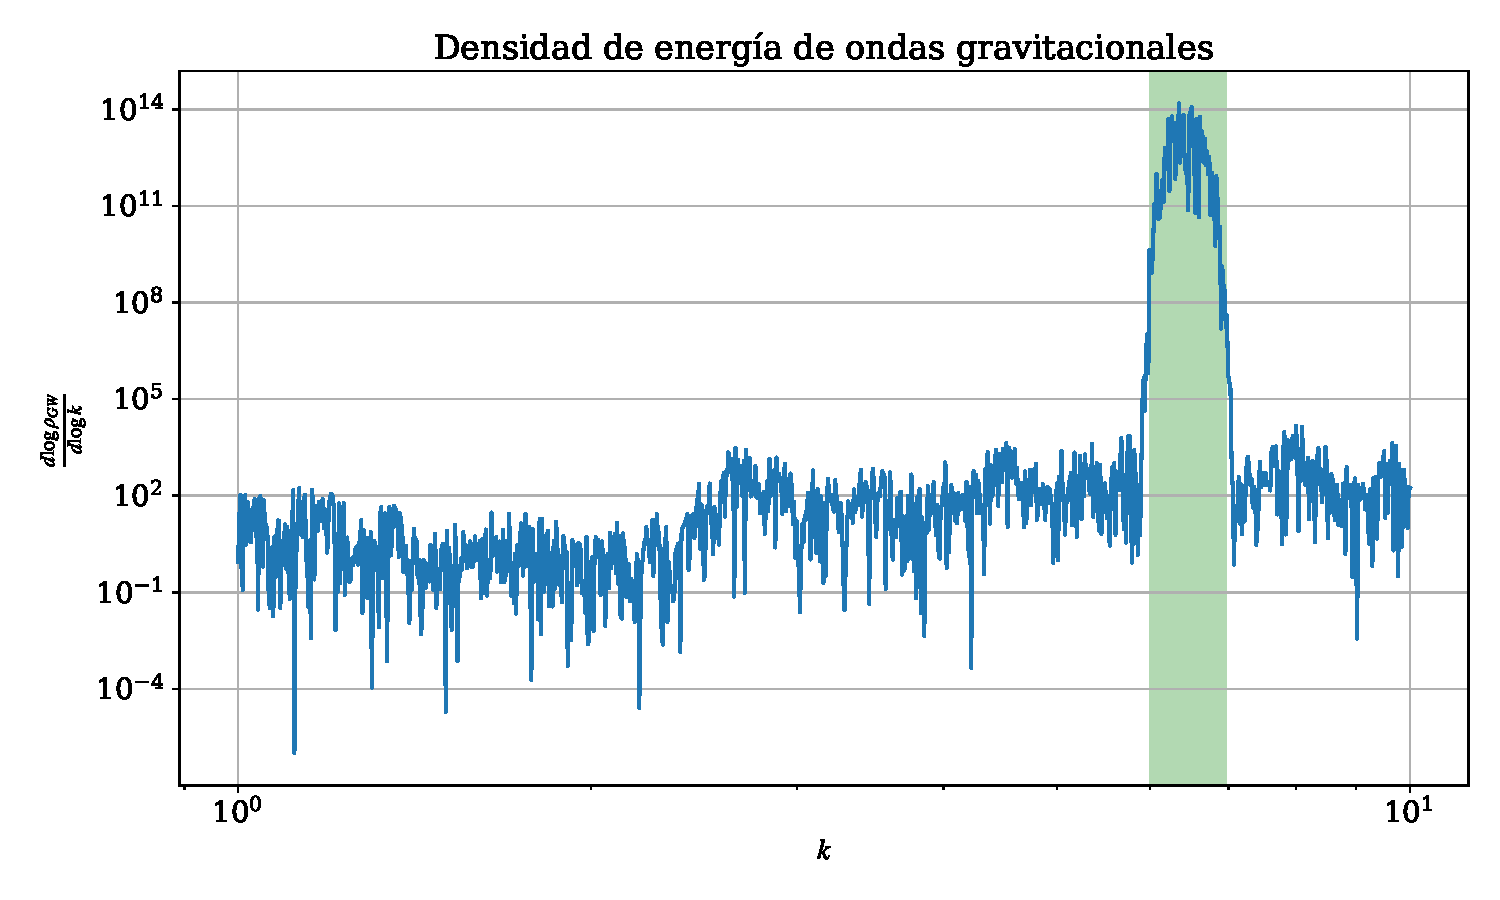
\includegraphics[width = 0.75\linewidth]{figures/rhoGW_lphi4(lineal).pdf}
    \caption{}
    \label{fig:GW_lineal}
\end{figure}